\chapter{Design}

\section{Prerequisite terms}

\begin{itemize}
  \item \textbf{SCTP packet} is the unit of data that is passed on to the
    lower layer protocol. It is composed of a common header followed by one or
    more chunks.

    \begin{figure}[h]
      \raggedleft
      \begin{bytefield}[bitwidth=1.0em]{32}
        \bitheader{0-31}\\
        \wordbox{1}{Common Header}\\
        \wordbox{1}{Chunk \#1}\\
        \wordbox{1}{\dots}\\
        \wordbox{1}{Chunk \#n}
      \end{bytefield}
      \caption{SCTP Packet Format}
    \end{figure}

  \item \textbf{SCTP Chunk} is a unit of information within an SCTP packet,
    containing either control information or user data. It consists of the
    following fields:

    \begin{itemize}
      \item \textbf{Chunk Type} identifies the type of information contained in
        the Chunk Value field. The chunk type values 16--62, 64--126, 129, 131,
        133--190, 194--254 are currently unassigned\cite{iana}.

        The highest-order 2 bits of this 8-bit field specify the action that
        must be taken if the processing endpoint does not recognize the Chunk
        Type.

        \begin{itemize}
          \item[\texttt{00 --}] Stop processing this SCTP packet and discard it.
          \item[\texttt{01 --}] Stop processing this SCTP packet and discard it
            and report the unrecognized chunk in an `Unrecognized Chunk Type'.
          \item[\texttt{10 --}] Skip this chunk and continue
            processing.
            \phantomsection
              \label{2bits}
          \item[\texttt{11 --}] Skip this chunk and continue processing,
            but report in an ERROR chunk using the `Unrecognized Chunk Type'
            cause of error.
        \end{itemize}

      \item \textbf{Chunk Flags} usage depends on the Chunk Type.
      \item \textbf{Chunk Length} represents the size of the chunk in bytes,
        including the Chunk Type, Chunk Flags, Chunk Length, and Chunk Value
        fields.
      \item \textbf{Chunk Value} contains the actual information to be
        transferred in the chunk.
    \end{itemize}

    \begin{figure}[h]
      \raggedleft
      \begin{bytefield}[bitwidth=1.0em]{32}
        \bitheader{0-31}\\

        \bitbox{8}{Chunk Type} &
        \bitbox{8}{Chunk Flags} &
        \bitbox{16}{Chunk Length}\\

        \wordbox{3}{Chunk Value}
      \end{bytefield}
      \caption{SCTP Chunk Format}
    \end{figure}

  \item Network Flow - A sequence of packets in a transport connection.

  \item Qdisc (Queueing Discipline) - An algorithm that manages the queue of a
    device, either egress or ingress. It can be either be classless or classful.
    Examples of classless qdiscs include FIFO, Token Bucket Filter (TBF) and
    Stochastic Fair Queuing (SFQ).
    Hierarchy Token Bucket (HTB) is one of the classful qdiscs.

  \item Classes - Some qdiscs can contain classes, which contain further qdiscs - traffic
       may  then  be enqueued in any of the inner qdiscs, which are within the
       classes.

\end{itemize}

\section{Send buffer value}
The kernel send buffer can be divided into 2 distinct parts:
\begin{itemize}
  \item unacknowledged in-flight segments.
  \item segments waiting to be sent (backlog).
\end{itemize}

\noindent
We propose to advertise the number of bytes in this backlog in the
Chunk Value field of the proposed chunk.
\begin{figure}[h]
  \centering
  \begin{bytefield}[bitwidth=1.0em]{32}
    \bitbox{16}{In-flight segments} &
    \bitbox{16}{Backlogged segments}
  \end{bytefield}
  \caption{Send buffer structure}
\end{figure}

\section{Previously Proposed Modification}
For advertising the send buffer occupancy, we propose to add a new Chunk Type,
with a 32-bit Chunk Value field containing the amount of backlogged data in the
send buffer.

To ensure that hosts running an unmodified SCTP stack skip this chunk without
returning an ERROR chunk, the highest-order 2 bits of the Chunk Type of this
chunk should be \texttt{10} (as explained in section~\ref{2bits}).
This limits the choice of the Chunk Type value between 128 and 190.

This chunk is sent at a specified interval.
The total size of this chunk is 8 bytes, which is 0.53\% of a typical
1500 byte packet.



\begin{figure}[h]
  \centering
  \begin{bytefield}[bitwidth=1.0em]{32}
    \bitheader{0-31}\\
    \bitbox{8}{Chunk Type} & \bitbox{8}{Chunk Flags} & \bitbox{16}{Chunk Length}\\
    \bitbox{32}{Send buffer size}
  \end{bytefield}
  \caption{Proposed Chunk for send buffer advertisement}
\end{figure}

\section{Currently Proposed Modification}
For advertising the send buffer occupancy, we propose to add a new Chunk Type,
with the Chunk Flags field containing the percentage occupancy of the send
buffer.

To ensure that hosts running an unmodified SCTP stack skip this chunk without
returning an ERROR chunk, the highest-order 2 bits of the Chunk Type of this
chunk should be \texttt{10} (as explained in section~\ref{2bits}).
This limits the choice of the Chunk Type value between 128 and 190.

Each SCTP packet contains this chunk as the first chunk.
The total size of this chunk is 4 bytes, which is 0.26\% of a typical
1500 byte packet.

\begin{figure}[h]
  \centering
  \begin{bytefield}[bitwidth=1.0em]{32}
    \bitheader{0-31}\\
    \bitbox{8}{Chunk Type} & \bitbox{8}{\scriptsize Percentage send buffer occupancy} & \bitbox{16}{Chunk Length}\\
  \end{bytefield}
  \caption{Proposed Chunk for send buffer advertisement}
\end{figure}

\section{Test bed design}
A dumbbell shaped network topology was created with two routers in the center,
and multiple hosts connected to one end of each router via a switch. This
ensures that we have a bottleneck link in all flows between end hosts on
either side.

\begin{figure}[h]
  \centering
  \small
  \begin{tikzpicture}[start chain=testbed going right]

    \node [on chain] {\vdots};

    \node [start branch=1 going above, on chain,
    label=below:PC\textsubscript{\(1\)}] (pc1)
    {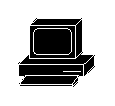
\includegraphics{imgs/pc.eps}};

    \node [start branch=2 going below, on chain,
    label=below:PC\textsubscript{\(x\)}] (pcn)
    {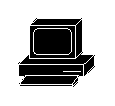
\includegraphics{imgs/pc.eps}};

    \node [on chain, join=with pc1, join=with pcn,
    label=below:Switch\textsubscript{\(1\)}]
    {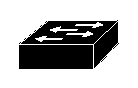
\includegraphics{imgs/switch.eps}};

    \node [on chain, join,
    label=below:Router\textsubscript{\(1\)}]
    {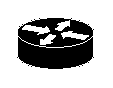
\includegraphics{imgs/router.eps}};

    \node [on chain, join,
    label=below:Router\textsubscript{\(2\)}]
    {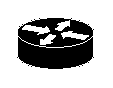
\includegraphics{imgs/router.eps}};

    \node [on chain, join,
    label=below:Switch\textsubscript{\(2\)}] (switch2)
    {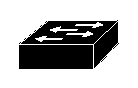
\includegraphics{imgs/switch.eps}};

    \node [on chain] {\vdots};

    \node [start branch=3 going above, on chain, join=with switch2,
    label=below:PC\textsubscript{\(x+1\)}]
    {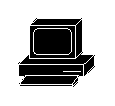
\includegraphics{imgs/pc.eps}};

    \node [start branch=4 going below, on chain, join=with switch2,
    label=below:PC\textsubscript{\(y\)}]
    {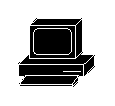
\includegraphics{imgs/pc.eps}};

  \end{tikzpicture}
  \caption{Test bed topology}
\end{figure}
